%----------------------------------------------------------------------------------------
%	PACKAGES AND THEMES
%----------------------------------------------------------------------------------------
\documentclass[aspectratio=169,xcolor=dvipsnames]{beamer}
\usetheme{SimplePlusAIC}

\usepackage{hyperref}
\usepackage{graphicx} % Allows including images
\usepackage{booktabs} % Allows the use of \toprule, \midrule and  \bottomrule in tables
\usepackage{svg} %allows using svg figures
\usepackage{tikz}
\usepackage{makecell}
\newcommand*{\defeq}{\stackrel{\text{def}}{=}}

%Select the Epilogue font (requires luaLatex or XeLaTex compilers)
\usepackage{fontspec}
\setsansfont{Epilogue}[
    Path=./epilogueFont/,
    Scale=0.9,
    Extension = .ttf,
    UprightFont=*-Regular,
    BoldFont=*-Bold,
    ItalicFont=*-Italic,
    BoldItalicFont=*-BoldItalic
    ]

%----------------------------------------------------------------------------------------
%	TITLE PAGE
%----------------------------------------------------------------------------------------

\title[Recognizability Embedding Enhancement for VLRFR \& QE]{Recognizability Embedding Enhancement for Very Low-Resolution Face Recognition and Quality Estimation} % The short title appears at the bottom of every slide, the full title is only on the title page
%\subtitle{Subtitle}

\author[Barbosa, Warley .V]{Warley Vital Barbosa}
%\institute[FEE CTU]{Artificial Intelligence Center \newline Faculty of Electrical Engineering\newline Czech Technical University in Prague}
% Your institution as it will appear on the bottom of every slide, maybe shorthand to save space

\AtBeginSection[]
{
  \begin{frame}{Overview}
  \tableofcontents[
    currentsection,
    sectionstyle=show/hide,
    subsectionstyle=show/show/hide
  ]
  \end{frame}
}

\date{\today} % Date, can be changed to a custom date
%----------------------------------------------------------------------------------------
%	PRESENTATION SLIDES
%----------------------------------------------------------------------------------------

\begin{document}

\begin{frame}[plain]
    % Print the title page as the first slide
    \titlepage
\end{frame}

\begin{frame}{Overview}
    % Throughout your presentation, if you choose to use \section{} and \subsection{} commands, these will automatically be printed on this slide as an overview of your presentation
    \tableofcontents
\end{frame}

%------------------------------------------------
\section{Introduction}
%------------------------------------------------

\begin{frame}{Real-World Scenarios}
    \begin{itemize} 
        \item In real-world face recognition deployment scenarios, the pixel resolution of the detected face images is significantly deflated;%, due to extreme long-range distance and broad viewing angle of the acquisition devices, especially in surveillance applications. 
        \item These tiny regions of interest are, in general, ranging from $16\times16$ to $32\times32$ pixels;% thereby suffering from poor pixel resolution, in addition to unrestricted noises such as poor illumination conditions, non-frontal poses with awful angles, unconstrained facial expressions, blurriness, and occlusions.
        \item Consequences
        \begin{itemize}
            \item Lack of generalizability because VLR face images undermine models trained on high-resolution (HR) images; 
            \item VLRFR models tends to fail to extract meaningful identity-specific patterns;
            \item Both issues are escalated due to ambiguous inter-class variations.
        \end{itemize}
        \item Challenges
        \begin{itemize}
            \item Same VLR resolution matching (VLR probe to a gallery set of the same resolution);
            \item Cross-resolution matching (HR galleries, VLR probes).
        \end{itemize}
    \end{itemize}
\end{frame}

%------------------------------------------------

\begin{frame}{Current methods for VLR FR}
    \begin{itemize}
        \item Most existing works designated for VLRFR improve the face quality of the VLR instances based on an auxiliary set of HR face images;
        \item Generic modes of operation
        \begin{itemize}
            \item \textbf{Image domain}: super-resolution, image synthesis;
            \item \textbf{Embedding domain}: resolution-invariant features, coupled mappings;
            \item \textbf{Classifier domain}: transfer learning, knowledge distillation.
        \end{itemize}
        \item Problems
        \begin{itemize}
            \item Most SoTA models require HR-VLR pairs, but in practice they are rare.
        \end{itemize}
    \end{itemize}
\end{frame}

%------------------------------------------------

\begin{frame}{Face Recognizability}
    \begin{itemize}
        \item \textbf{Face Recognizability} (also known as face quality) represents how well a face image is for discrimination purposes;% face quality is closely related too face recognition performance
        \item Some works focus on Face Image Quality Assessment (FIQA)---predicting a face image's suitability for face recognition;
        \item In this context, there are two ways of predictions
        \begin{itemize}
            \item Label the training data with face image quality scores and solve a regression problem;
            \item Link the face embedding properties to FIQ scores.
        \end{itemize}
        \item The second approach seems better, but could be improved if the FIQ scores were learned.
    \end{itemize}
\end{frame}

%------------------------------------------------

\begin{frame}{Face Recognizability}
    \begin{itemize}
        \item Deng (2023) reported that deep learning-based face model induces an \textbf{unrecognizable cluster} in the embedding space.
    \end{itemize}
    \begin{figure}
        \centering
        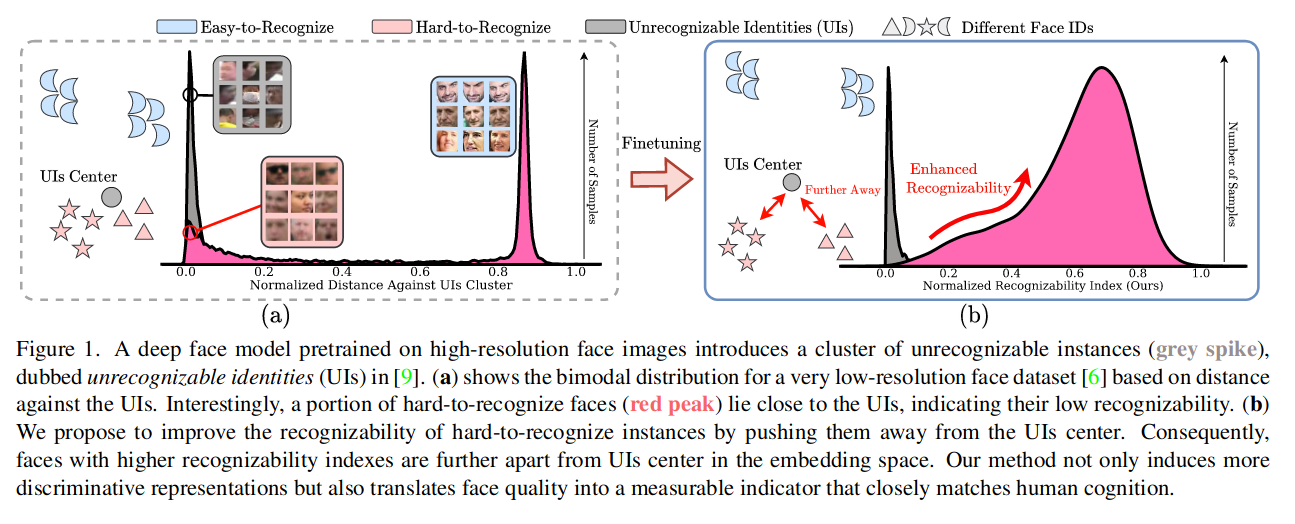
\includegraphics[width=0.7\textwidth]{imgs/01_Recognizability.png}
        \caption{Chai (2023)}
        \label{fig:recognizability}
    \end{figure}
\end{frame}
%------------------------------------------------

\begin{frame}{Proposal}

    \begin{alertblock}{Proposal}
        Elevate the recognizability of every VLR face embedding;
    \end{alertblock}
    \begin{enumerate}
        \item A learning-based recognizability index (RI) computes the cosine proximity of each embedding with the UIs cluster and the associated positive and negative prototypes;
        \item An index diversion (ID) loss detaches the hard-to-recognize embeddings from the UIs cluster;
        % We underline that embedding learning in the direction opposing the UIs contributes to a higher explanatory power whilst promoting inter-class separation, particularly for hard-to-recognize instances.  \textbf{}
        \item And a perceptibility attention mecanism which attends to meaningful face regions.
    \end{enumerate}
\end{frame}
%------------------------------------------------
\begin{frame}{Contributions}
    \begin{enumerate}
        \item A novel approach to VLRFR that uses the face recognizability notion in the embedding space to improve the hard-to-recognize instances;
        \item A robust learning-based face recognizability measure---it uses face embeddings intrinsic proximity relationship against the UIs cluster with class prototypes;
        \item A index diversion loss to enhance RI and a perceptibility attention mechanism to focus on the most salient face regions;
        \item More discriminative embedding space for VLRFR, but also a recognizability-aware embedding learning and face recognizability estimation.
    \end{enumerate}    
\end{frame}
%------------------------------------------------
\section{Related Works}
%------------------------------------------------

\begin{frame}{VLRFR}
    \begin{itemize}
        \item Existing HR image dependence approaches for VLRFR can be categorized into image domain, embedding domain, and classifier;
        \begin{itemize}
            \item \textbf{Image domain}---super-resolution learns a mapping function to upscale VLR to HR; %Several works relate recognition to visual quality, but they need mated HR-VLR pairs.
            \item \textbf{Embedding domain and classifier levels}---most knowledge distillation approaches aimed to transfer the knowledge of the HR domain to the VLR face model. 
        \end{itemize}
        \item This work involves no auxiliary HR images--improvements are focused on recgonizability rather than visual quality.
    \end{itemize}
\end{frame}

%------------------------------------------------

\begin{frame}{FIQA}
    \begin{itemize}
        \item Face Image Quality Assessment (FIQA) can be mainly divided into two categories:
        \begin{itemize}
            \item The first category is to solve a regression problem to assess the training images with FIQ scores---human quality annotation, similarity between random positive mated pairs, etc.
            \item The second category directly utilizes intrinsic properties of face embeddings to estimate face quality without explicit regression learning---robustness of stochastic embeddings, uncertainty variation, embedding norm, etc.
        \end{itemize}
        \item Aside from face quality, several works also explore classifiability according to face quality;
        % While most FIQA methods struggle to learn adaptive margins for competent quality-aware embedding...
        \item This work strives to improve embedding learning based on the proposed RI---it demonstrates that RI characterizes the image quality better, and its model can extract meaningful semantics important to face recognition.
    \end{itemize}
\end{frame}

%------------------------------------------------
\section{Methodology}
%------------------------------------------------
\begin{frame}{Recognizability Index (RI) Formulation}
   \begin{itemize}
       \item There is a relationship between face quality and recognition performance---here it is quantified by intra-class and inter-classes similarity measures;
       \item Face quality, defined here as the Recognizability Index $\xi_i$, can be estimated from the proximity of each instance with respect to its positive and negative prototypes relative to the UIs center
       %\begin{itemize}
       %    \item Instances close to the UIs are the hard-to-recognize samples;
       %    \item That is, they have the smallest proximity $d^{UI}_i$ between an instance's $i$ L2-normalized embeddings $\hat{v}_i$ and the UIs cluster center $\bar{v}_{UI}$. 
       %\end{itemize}
       $$\xi_i = d_{i}^{UI} \frac{d_i^N}{d_i^P + \epsilon}$$
   \end{itemize} 
\end{frame}
%------------------------------------------------
\begin{frame}{Perceptibility Regression Module}
    \begin{figure}
        \centering
        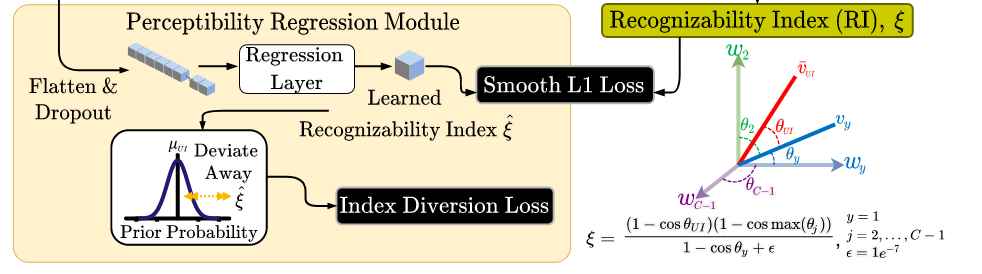
\includegraphics[width=0.7\textwidth]{imgs/12_Fig_3_3_PRM.png}
        \label{fig:f3-3-prm}
    \end{figure}
   \begin{itemize}
    %\item The model serves recognizability-aware embedding learning and quality estimation simultaneously, which explains the perceptibility regression module below.
    \item The predicted and learnable RI, denoted by $\hat{\xi}$, is matched to $\xi_i$ via smooth L1 loss% This loss changes to L2 and vice-versa depending on the regression error interval
    $$L_{L1} = 
    \begin{cases}
        0.5 (\xi_i - \hat{\xi_i})^2 & \text{if} |\xi_i - \hat{Xi_i}| < \beta\\
        |\xi_i - \hat{\xi_i}| - 0.5 \times \beta & \text{otherwise}
    \end{cases}
    $$
    %\item Differently from Embedding Recognizability Score (Deng et al., 2023), the RI considers the intra-class and inter-class proximities, and doesn't require the UIs cluster center to be known
    %\begin{itemize}
    %    \item The regression module incorporates the proximity relation.
    %\end{itemize}
   \end{itemize} 
\end{frame}
%------------------------------------------------

%------------------------------------------------
\begin{frame}{Index Diversion Loss}
   \begin{itemize}
    \item They assume the RI distribution of the UIs cluster follows the standard Gaussian distribution with $\mathcal{N}(0, 1)$;
    %\begin{itemize}
    %    \item It has better interpretrability and a more stable RI;%than it would have if they estimate the mean and variance of the Gaussian by forwarding the UIs through the perceptibility regression module. 
    %    \item It enhances the hard-to-recognize instance's recognizability via an statistical diversion of the estimated RI.
    %\end{itemize}
    \item The diversion is the standardized estimated RI with respect to $\mu_{UI}$ and $\sigma_{UI}$ of the UI distribution $$div = \frac{\hat{\xi_i} - \mu_{UI}}{\sigma_{UI}}$$
    which becomes the Index Diversion Loss $$L_{ID} = \text{max}(0, \tau - div)$$
   \end{itemize} 
\end{frame}

%------------------------------------------------
\begin{frame}{Perceptibility Attention Module}
    \begin{figure}
        \centering
        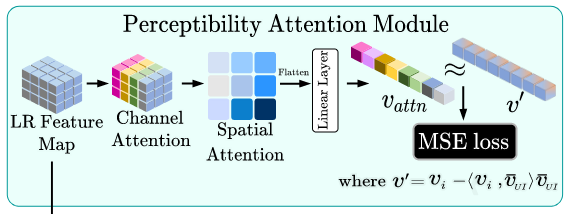
\includegraphics[width=0.4\textwidth]{imgs/11_Fig_2_2_PAM.png}
        \label{fig:f2-2-pam}
    \end{figure}
    \begin{itemize}
        \item They conjecture that an orthogonal projection of a VLR face instance $v_i$ onto the L2-normalized UIs cluster center $\bar{v_{UI}}$ by an attention module helps the model to learn meaningful features for recognizability;
        %\begin{itemize}
        %    \item They argue the module guides the model to attend to richer interpretative contents important to recognition purposes. 
        %\end{itemize}
        \item The learned projection is optimized with the mean square error loss
        $$L_{MSE} = \frac{1}{B} \sum_{i=1}^B (\mathbf{v_i'} - \mathbf{v_i}^{attn})^2$$
        thus formalizing the problem as a regression.
    \end{itemize}
\end{frame}
%------------------------------------------------

%------------------------------------------------
\begin{frame}{Proposed Model}
    \begin{figure}
        \centering
        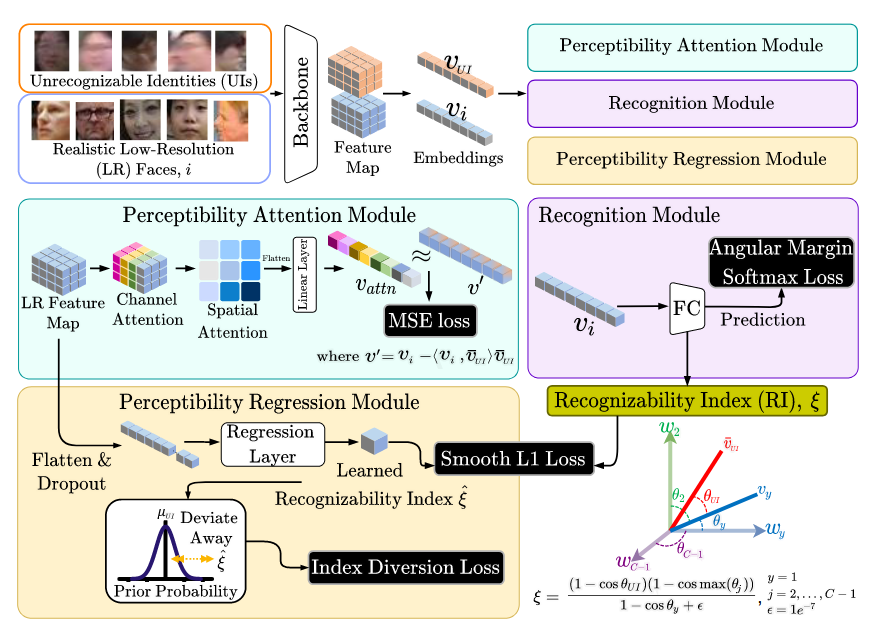
\includegraphics[width=0.5\textwidth]{imgs/10_Fig_2_1_Method.png}
        \label{fig:f2-1-method}
    \end{figure}
    \begin{itemize}
        \item The overall loss is a weighted sum of four loss, including the ArcFace as the classification loss
        $$L_{total} = L_{cls} + \alpha L_{L1} + \beta L_{ID} + \gamma L_{MSE}$$
    \end{itemize}
\end{frame}
%------------------------------------------------

%------------------------------------------------
\section{Experiments and Results}
%------------------------------------------------

\begin{frame}{Datasets, Models, and Metrics}
    \begin{itemize}
        \item Datasets
        \begin{itemize}
            \item They benchmarked against TinyFace, SurvFace, and SCFace via the open-set evaluation protocol;
            \item An unlabeled UI face dataset was built to generate UIs cluster.
        \end{itemize}
        \item Models
        \begin{itemize}
            \item The MobileFaceNet and ResNet50 models were pretrained on the VGGFace2 and finetuned on the respective benchmark datasets;
            \item Their baseline was the models trained with ArcFace loss.
        \end{itemize}
        \item Metrics
        \begin{itemize}
            \item For TinyFace and SCFace, they used rank-1 identification rate (IR) \%;
            \item For SurvFace, they used TPIR @ FPIR and TPR @ FAR due to the inclusion of non-mated face images in its testing set; 
            \item For face image quality, they provide Error versus Reject Curve (ERC), False Non-Match Rate (FNMR) @ False Match Rate (FMR).
        \end{itemize}
    \end{itemize}
\end{frame}

%------------------------------------------------

\begin{frame}{Comparison with SoTA Methods}
    \begin{itemize}
        \item They argue that their proposed method is robust against the resolution gap in VLR-HR matching, as well as a viable solution to the downstream VLR-VLR task;
        \item However, there is a space for KD and resolution invariant methods without finetuning on the VLR datasets---they are prone to overfitting.
    \end{itemize}
\end{frame}

%------------------------------------------------

\begin{frame}{Comparison with SoTA Methods}
    \begin{figure}
        \centering
        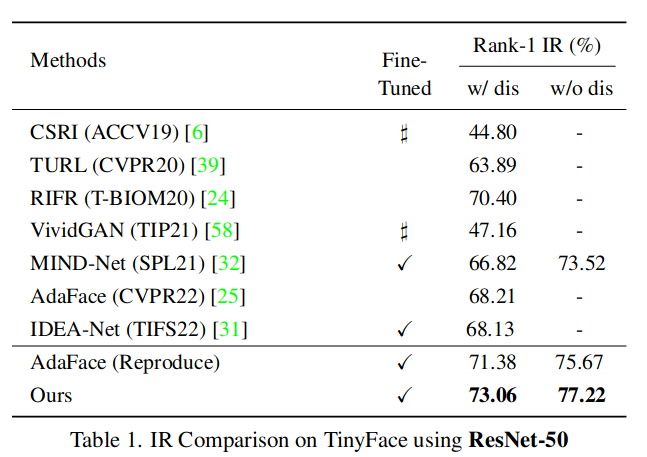
\includegraphics[width=0.5\textwidth]{imgs/02_Table_1_TinyFace.png}
        \label{fig:t1-tinyface}
    \end{figure}
    \begin{itemize}
        \item Improving recognizability at the feature level is more meaningful than super-resolving the visual quality of the VLR face images.
    \end{itemize}
\end{frame}

%------------------------------------------------

\begin{frame}{Comparison with SoTA Methods}
    \begin{figure}
        \centering
        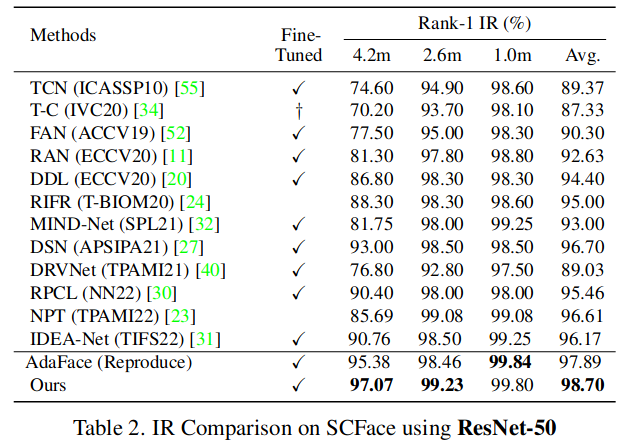
\includegraphics[width=0.4\textwidth]{imgs/03_Table_2_SCFace.png}
        \label{fig:t2-scface}
    \end{figure}
    \begin{itemize}
        \item The enhanced recognizability bridges the resolution gap between the HR and the VLR face features;
        \item The attention module singles out the most salient regions from VLR and HR faces, resulting in better cross-resolution matching scores.% especially for the face images captured from 4.2m (the largest standoff distances compared to 1.0m and 2.6m
    \end{itemize}
\end{frame}

%------------------------------------------------

\begin{frame}{Comparison with SoTA Methods}
    \begin{figure}
        \centering
        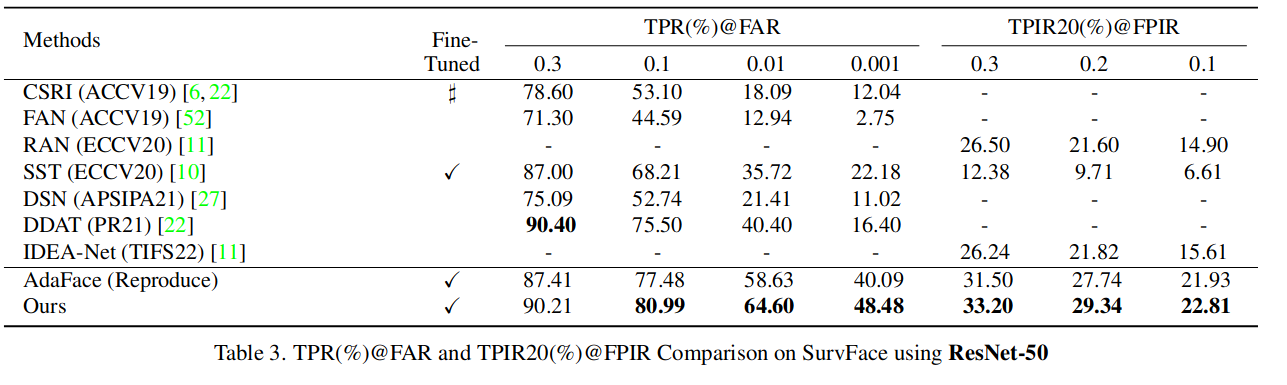
\includegraphics[width=0.7\textwidth]{imgs/04_Table_3_SurvFace.png}
        \label{fig:t3-survface}
    \end{figure}
    \begin{itemize}
        \item On the the most challenging dataset, they outperform other SoTAs under the most rigorous settings, which shows that their method is very robust. 
        %\item They also point out that none of them "resolves the VLRFR by means of refining feature recognizability". 
    \end{itemize}
\end{frame}


%------------------------------------------------

\begin{frame}{Ablation Analysis}
    \begin{figure}
        \centering
        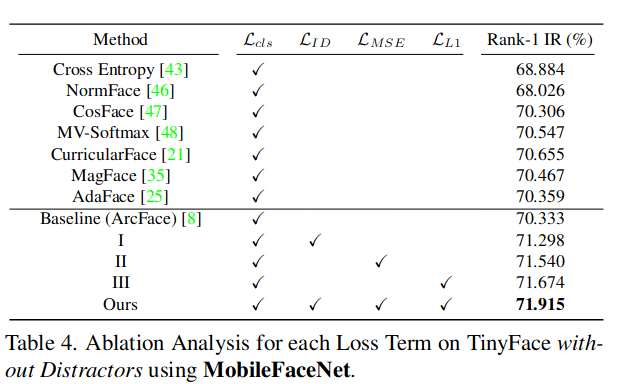
\includegraphics[width=0.5\textwidth]{imgs/05_Table_4_AA.png}
        \label{fig:t4-aa}
    \end{figure}
    \begin{itemize}
        %\item It is believed that learning the softmax prototypes simultaneously with the RI prompts the model to encode the embedding recognizability at each training step. 
        \item The learned RI can be viewed as an index of the model’s confidence corresponding to the classifiability of any face image, including the unknown instances.
    \end{itemize}
\end{frame}

%------------------------------------------------

\begin{frame}{Ablation Analysis}
    \begin{figure}
        \centering
        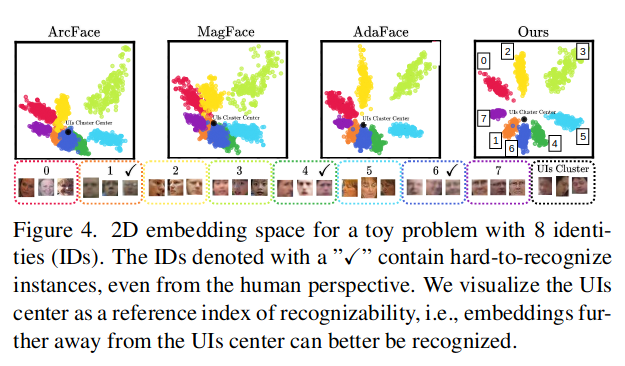
\includegraphics[width=0.5\textwidth]{imgs/06_Fig_4_AA.png}
        \label{fig:f4-aa}
    \end{figure}
    \begin{itemize}
        %\item It is discerned that the competing models are incapable of separating the hard-to-recognize clusters from the UIs center. 
        \item Their model is inclined to divert the hard-to-recognize instances from the UIs center, yielding a well-separable (therefore a more discriminative) embedding space to resolve the downstream VLRFR task.
    \end{itemize}
\end{frame}

%------------------------------------------------

\begin{frame}{Ablation Analysis}
    \begin{figure}
        \centering
        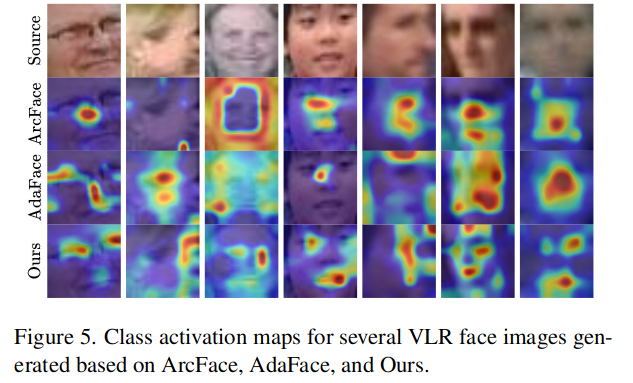
\includegraphics[width=0.5\textwidth]{imgs/07_Fig_5_AA.png}
        \label{fig:f5-aa}
    \end{figure}
    \begin{itemize}
        \item Attending to the embeddings away from the UIs center focuses more on the salient face features, i.e. eyes, nose, and mouth, even when the face images appear to be obscure.
    \end{itemize}
\end{frame}


%------------------------------------------------

\begin{frame}{Face Image Quality Assessment}
    \begin{figure}
        \centering
        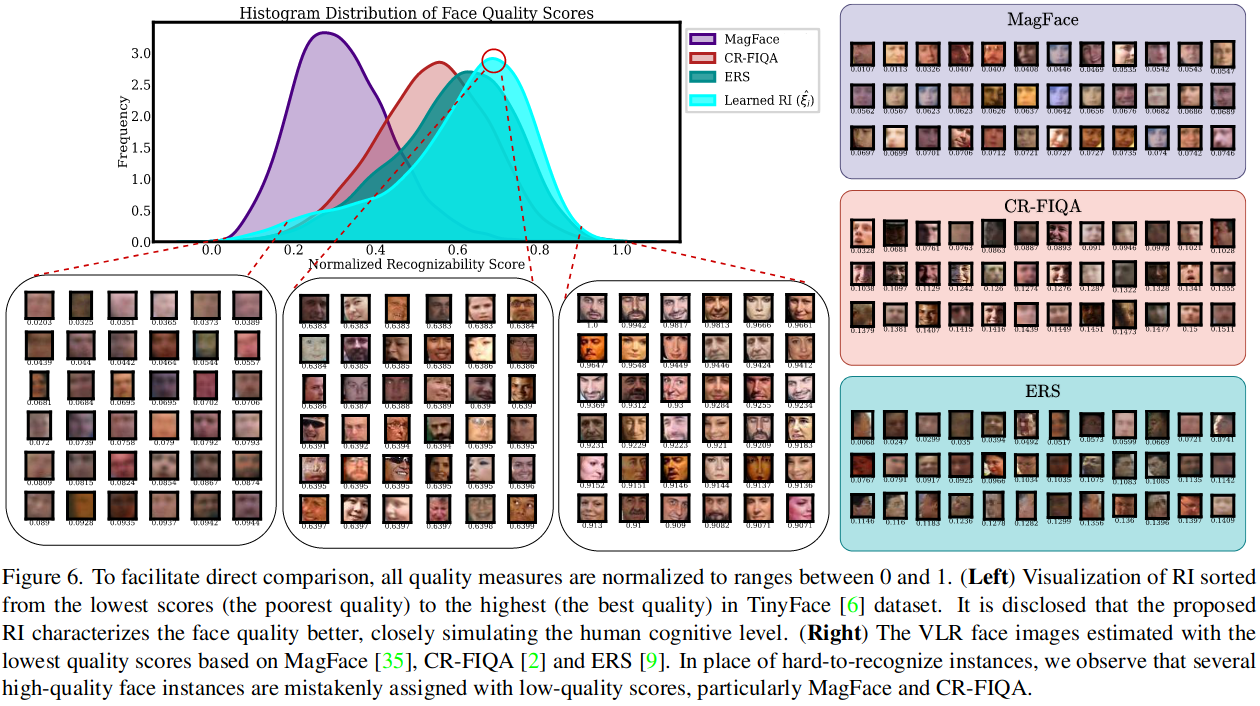
\includegraphics[width=0.75\textwidth]{imgs/08_Fig_6_AA.png}
        \label{fig:f6-aa}
    \end{figure}
    \begin{itemize}
        \item ID loss improves recognizability by skewing the RI distribution, thus showing that the RI is a robust indicator of recognizability.
    \end{itemize}
\end{frame}

%------------------------------------------------

\begin{frame}{Face Image Quality Assessment}
    \begin{figure}
        \centering
        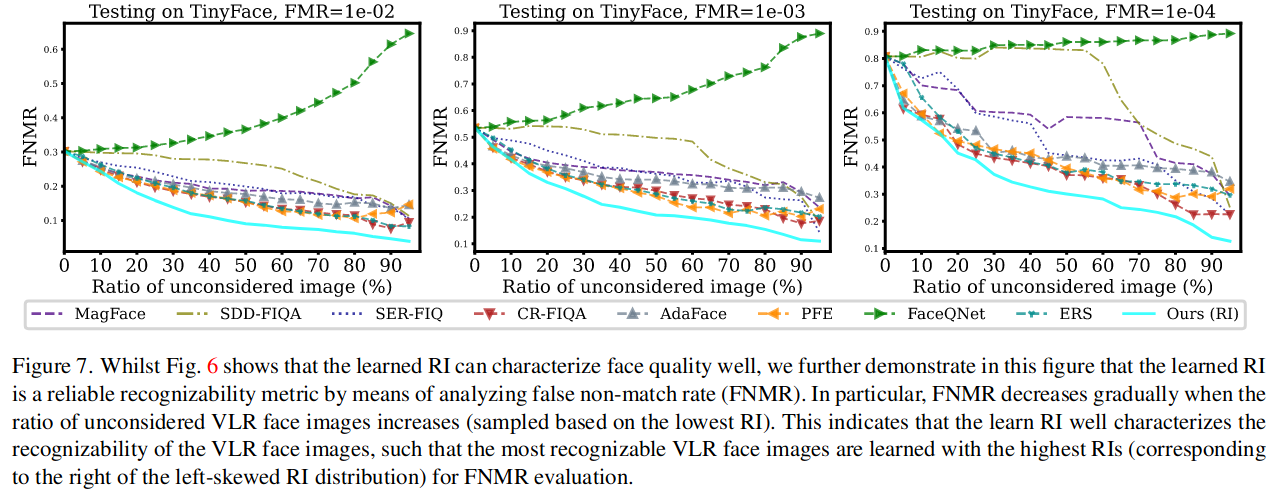
\includegraphics[width=0.7\textwidth]{imgs/09_Fig_7_AA.png}
        \label{fig:f7-aa}
    \end{figure}
    \begin{itemize}
        \item A subsequent verification task on TinyFace shows that the learned RI outperforms SoTA in Error vs Rejection Rate---the error decreases as the ratio of unconsidered image decreases.
    \end{itemize}
\end{frame}


%------------------------------------------------
\section{Conclusion}
%------------------------------------------------
\begin{frame}{Conclusion}
    \begin{itemize}
        \item This paper addresses the problem arising from the hard-to-recognize faces in VLR images 
        \begin{itemize}
            \item Rather than treating these faces as UIs, the authors take a principled recognizability notion to characterize the recognizability of each image with a robust indicator, specifically the recognizability index (RI).
        \end{itemize}
        \item Interestingly, attending to the embeddings projected away from the UIs cluster provides more explanatory power to the model to highlight the facial features more precisely.
    \end{itemize}
\end{frame}

%------------------------------------------------
\begin{frame}{References}
    % Beamer does not support BibTeX so references must be inserted manually as below
    \footnotesize{
        \begin{thebibliography}{99}
            \bibitem[Chai, 2023]{p1} Chai et al. (2023)
            \newblock Recognizability Embedding Enhancement for Very Low-Resolution Face Recognition and Quality Estimation
            \newblock \emph{arXiv preprint} arXiv:2304.10066
        \end{thebibliography}
    }
    \footnotesize{
        \begin{thebibliography}{99}
            \bibitem[Deng, 2023]{p1} Deng et al. (2023)
            \newblock Harnessing Unrecognizable Faces for Improving Face Recognition
            \newblock 2023 IEEE/CVF Winter Conference on Applications of Computer Vision (WACV)
        \end{thebibliography}
    }
\end{frame}

%------------------------------------------------

\begin{frame}
    \Huge{\centerline{\textbf{The End}}}
\end{frame}

%----------------------------------------------------------------------------------------
\end{document}